\chapter{Methods implemented in \comus} %\label{chap:features}

\section{Hudson's ms mode}

\subsection{Infinite Site Model simulations}

Since \comus\ is using the Hudson's ms implementation to build the coalescent tree, it preserves most of the functionality of ms (at the moment the split of a population backwards in time, i.e. the -s option, is not supported). Thus, the user can use the exact command line of ms to generate polymorphic data under the Wright-Fisher and infinite site model. 

For example:

\begin{lstlisting}
  ./comus 10 1000 -t 10 -r 100 100
\end{lstlisting}

will produce a sample of polymorphic sites given that the population mutation rate is 10 and the population recombination rate is 100. 

For further information, please consult the manual of ms (\url{http://home.uchicago.edu/rhudson1/source/mksamples.html}).

\subsection{Finite Site Model simulations}

Finite site model simulations is a new feature of \comus.  A lot of the code used for the finite site model implementation has been implemented in the Seq-Gen package \citep{Rambaut1997}. Thus, \comus\ is able to handle various evolutionary mutation models such as the HKY, GTR, JC etc. An example command line is the following:

\begin{lstlisting}
  ./comus 1 2 1000 -t 10 -r 100 100 -mm hky -msites 10 
  -name myFirstRun -oCoalescent
\end{lstlisting}

This command line will produce sequences of length 10 (\verb!-msites 10!), under the HKY (\verb!-mm hky!) model. There is recombination (\verb!-r 100 100!)and a file with the coalescent trees will be produced (\verb!-oCoalescent!). Note, that you should provide the number of species that you simulate (here, this is the \verb!1! after the \verb!./comus!). Also, you should provide a name for the specific run (\verb!-name myFirstRun!). This name will be used as a suffix to the produced files (e.g. alignment file, info file, or coalescent file). 

\subsection{Substitution rate heterogeneity among sites}
Substitution rate heterogeneity among sites has been implemented using the source code of seq-gen. The rate heterogeneity model assigns a different substitution rate to each site according to a gamma distribution. The mean rate for all sites is 1.0, that is the gamma distribution is scaled. However, the user should provide the $\alpha$ parameter of the gamma distribution, i.e., should provide the shape parameter. Low values for the shape parameter simulate large heterogeneity. Contrary, large $\alpha$ values simulate homegeneity of substitution rates between sites. Gamma distribution can be continuous, or it can be approximated by a discrete function, where a finite number of rate categories (provided by the user) exist. 

The relevant command line flags are the following:

\begin{itemize}
\item \verb!-alpha!: The alpha parameter of the gamma distribution
\item \verb!-gammacategories!: How many rate-heterogeneity categories should exist (this generates a discrete model).
\end{itemize}

If only the \verb!-alpha! argument is used, and {\bf not} the \verb!-gammacategories!, then the model is assumed to be continuous. 


\subsection{Invariable sites}
Similarly to Seq-Gen, CoMuS implements an invariable sites model. With the invariable sites model, a proportion (given by the user) of sites {\bf are expected} to be invariable across the whole tree. The expected number of substitutions then, are falling into the remaining `potentially variable' sites. 

For further information please consult the manual of Seq-Gen (\url{http://bioweb2.pasteur.fr/docs/seq-gen/}). 


\section{Multiple species simulations}

In contrast to Hudson's ms, \comus\  is able to simulate samples from multiple species, i.e. it can simulate simultaneously intra- and inter-species genomic variability. To achieve that it uses ms' machinery, treating different species as isolated populations. On top of that, \comus\ can either produce polymorphic data using the infinite site model, or it can produce sequence data under the finite site model. A guide phylogenetic tree (provided as an input or simulated under various birth-death models) specifies the species limits.

\subsection{ The guide phylogenetic tree }

Assume a {\bf phylogenetic tree } of Figure \ref{fig:1}.


\begin{figure}[htbp!]
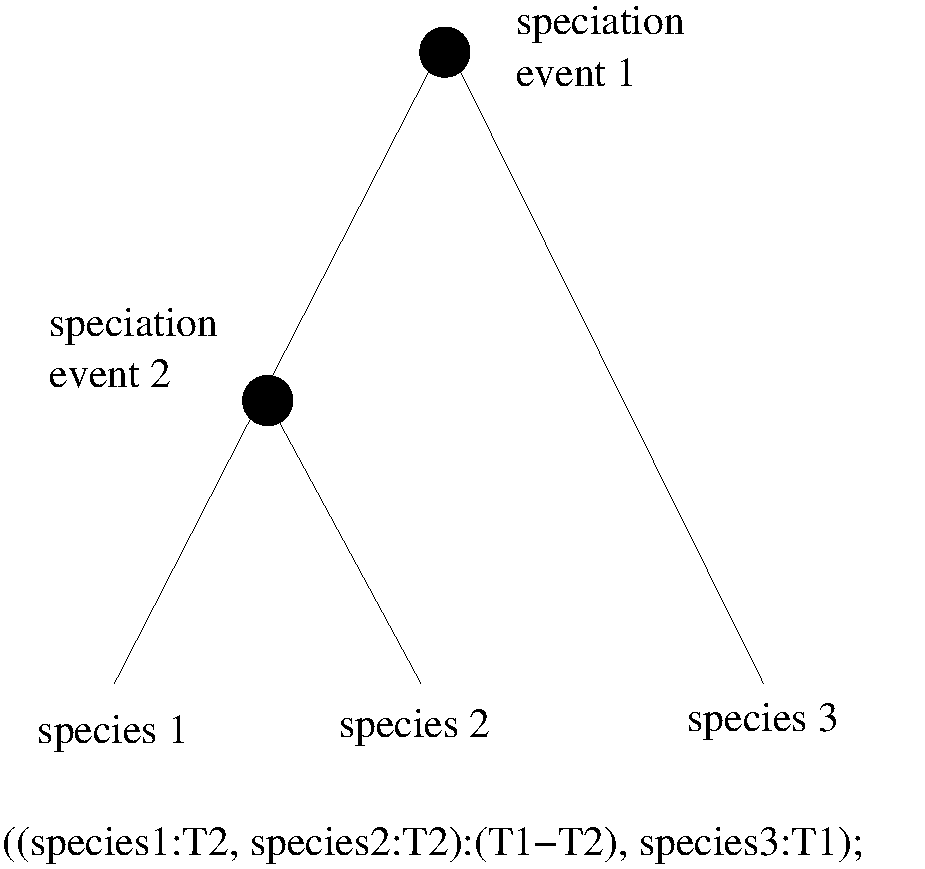
\includegraphics[width=0.5\textwidth]{guideTree.pdf}
\caption{A guide {\bf rooted} phylogenetic tree, used to specify the species limits for \comus\ simulations. There are two speciation events. Event 1 is more ancestral (at T1) and denotes a creation of two species, species 3 and the ancestral of species 1 and 2. Then, at time T2, a new speciation event took place, and species 1 and 2 are created. At the bottom, you can see the newick format of the tree. Each parenthesis represents a node. The lengths T1 and T2, represent the age of the two internal nodes of the tree. Finaly, the number after the ':' symbol represents the length of the branch above the specific node. Thus, the length of the branch that connects speciation 1 with speciation 2 is $T1 - T2$. }
\label{fig:1}

\end{figure}

Based on the guide tree, \comus\ will obtain the speciation times $T1$ and $T2$ and will treat them as a forward in time split, or backward in time joint between populations. In ms, this process is marked by the \verb!-ej! flag. If each species contains just a single population, the case is quite simple, since at each speciation time, the populations just merge as we go backwards in time. In case that there are more populations per species, the situation is more complicated; see below for details. 


\subsection{ Working with populations instead of species }
Since coalescent theory has been developed for populations and not for species (i.e. the structured coalescent model), we try to represent species as a set of populations that may remain isolated for a period of time. For example in Figure \ref{Fig:2}, we see two species (in blue and yellow). By convention, yellow species is assumed to be ancestral, and the blue species is created at time 'speciation'. The blue species comprises two populations that were created instantaneously at speciation time. To describe this process backward in time, we need to merge all populations at speciation time, since at this time point and proceeding backwards, the populations are not independent but they all belong to the same species and in one panmictic population. 

Populations are treated as in Hudson's ms. At speciation time points, we follow two approaches:
\begin{itemize}
\item In \comus, we put an index on each population and, at speciation time, all populations merge to the population with the largest index (Figure \ref{fig:2}). 
\item If the user has created a population merge event in the command line, then \comus\ acts according to the command line, \emph{even though the merge dictated by the command line is older than the speciation event}. I cannot find any relevant biological example, but there might exist some (Figure \ref{fig:3}). 
\end{itemize}
  
\begin{figure}[htbp!]

  \begin{subfigure}{0.5\textwidth}
    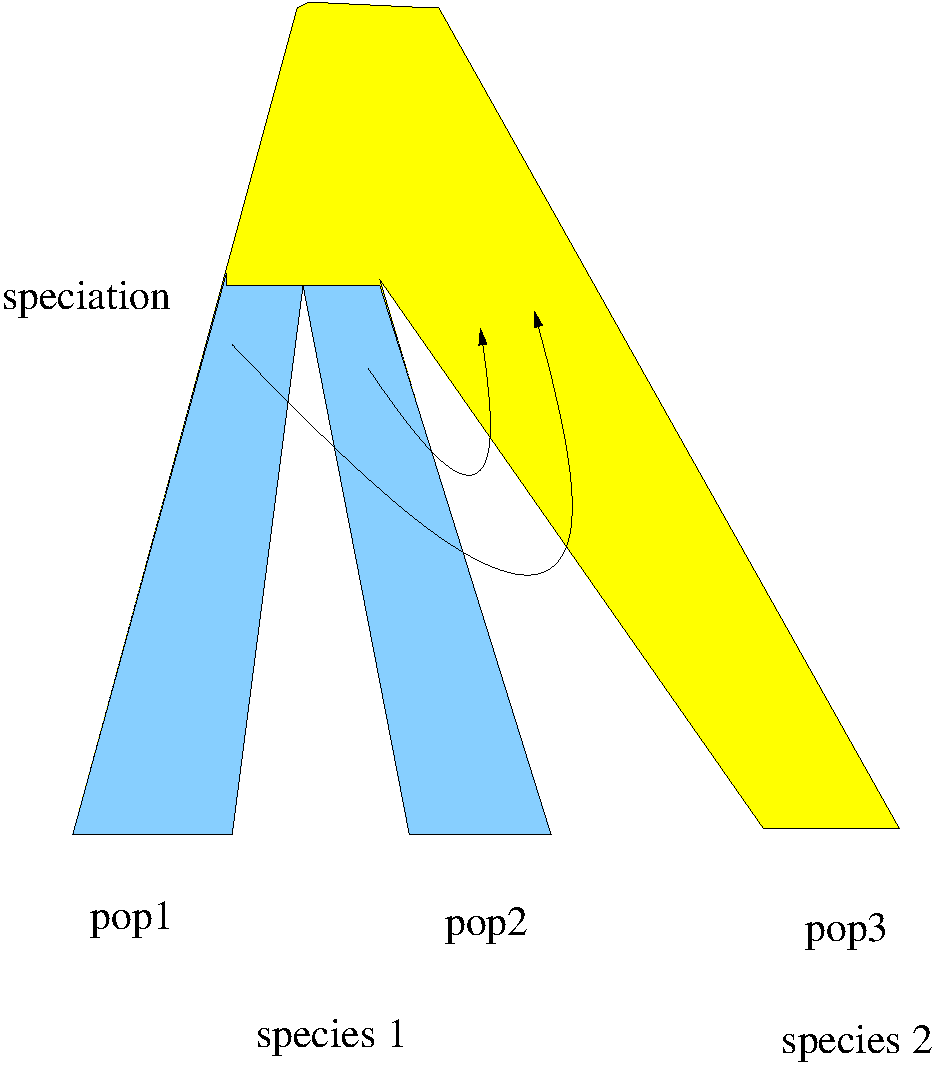
\includegraphics[width=\textwidth]{popmerge.pdf}
    \caption{}
    \label{fig:2}
  \end{subfigure}
  \begin{subfigure}{0.5\textwidth}
    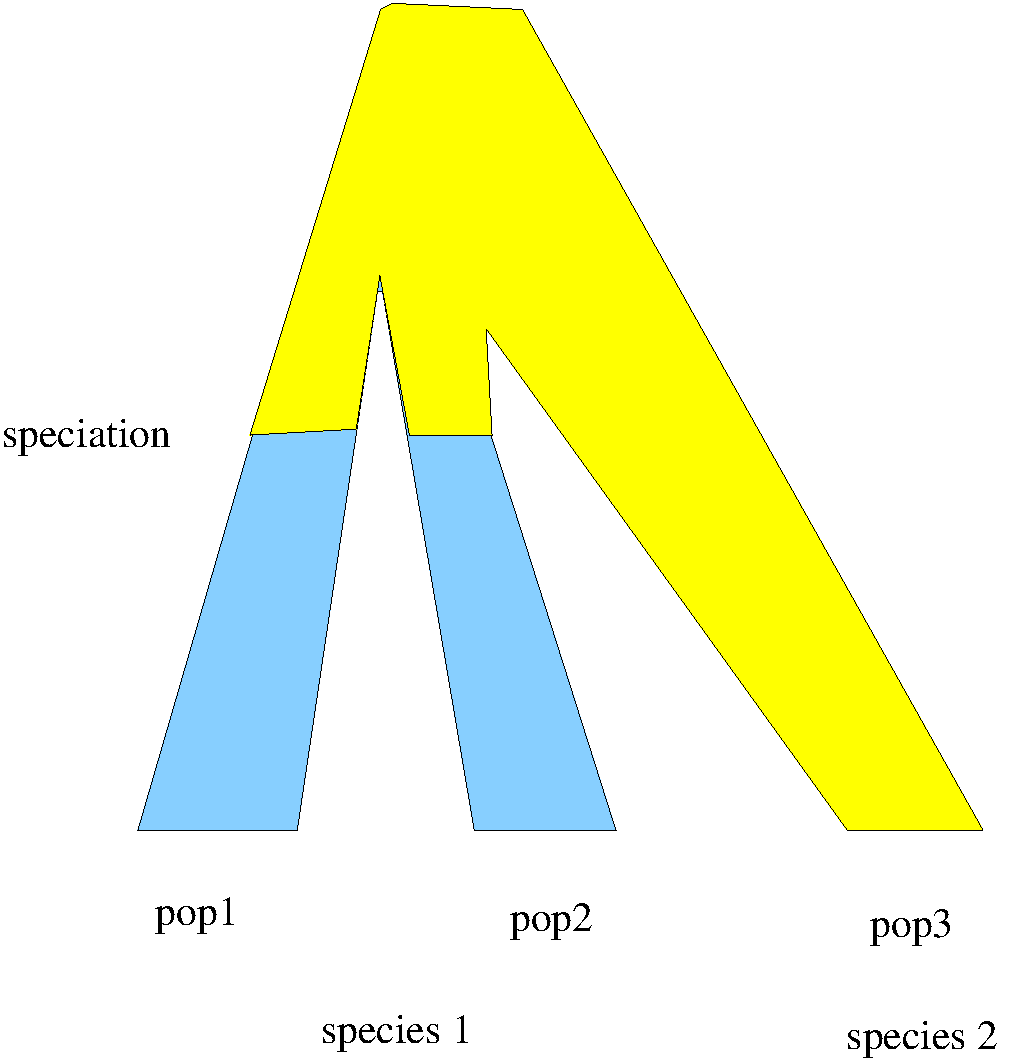
\includegraphics[width=\textwidth]{popmerge2.pdf}
    \caption{}
    \label{fig:3}
  \end{subfigure}
  \caption{Modeling species with multiple populations in \comus. In \ref{fig:2}, a species (yellow) splits in two (yellow and blue) and instantly the blue species, splits in two populations. Backwards in time, by convention, all populations merge with the population with the greatest index at speciation time. In \ref{fig:3}, we allow the user to define population merge events in command line (using the {\it -ej} option) that are independent of speciation events. Thus, pop1 merges with pop2 at a time which is older than the speciation event}
\end{figure}



\subsubsection{Examples}

The command line \ref{cmd:1} produces the alignment shown in Figure \ref{fig:5}. In Figure \ref{fig:5}, two species are simulated, each with 5 sequences. The first species comprises two populations, with 3 and 2 sequences, respectively. The second species consists of one population. Population 1 and population 2, from species 1, split at speciation time and remain isolated from each other till present. Thus, divergence between them is as large as divergence between species 1 and 2. 

\begin{lstlisting}[label=cmd:1, caption={Command line to produce model of figure \ref{fig:2}}]{language=bash, label=cmd:1}
  ./comus 2 5 5 1 -I 1 2 3 2 -t 10 -mm hky 
  -birth 2 -name example1
\end{lstlisting}

The command line \ref{cmd:2}, produces the alignment shown in Figure \ref{fig:5}. In this case, populations 1 and 2 from species 1 remain isolated even after (backwards) isolation. At speciation time, then, we apply the following convention:

\begin{itemize}
\item Starting from the population with the smallest index (here population 1 from species 1), we merge each population to the population with the greatest index (here, this is population 3 from species 2) unless there is a conflict obtained by the command line.
\end{itemize}

Here, since we merge population 1 with population 3, we cannot merge population 2 with population 3 because population 1 and population 2 should stay isolated until the time defined on the command line.

\begin{lstlisting}[label=cmd:2, caption={Command line to produce the model of figure \ref{fig:3}}]{language=bash, label=cmd:2}
  ./comus 2 5 5 1 -I 1 2 3 2 -t 10 -mm hky -birth 2 
  -name example2 -ej 2.0 1 2 1 -oPhylo -oCoalescent
\end{lstlisting}

\begin{figure}[htbp!]

  \begin{subfigure}{\textwidth}
    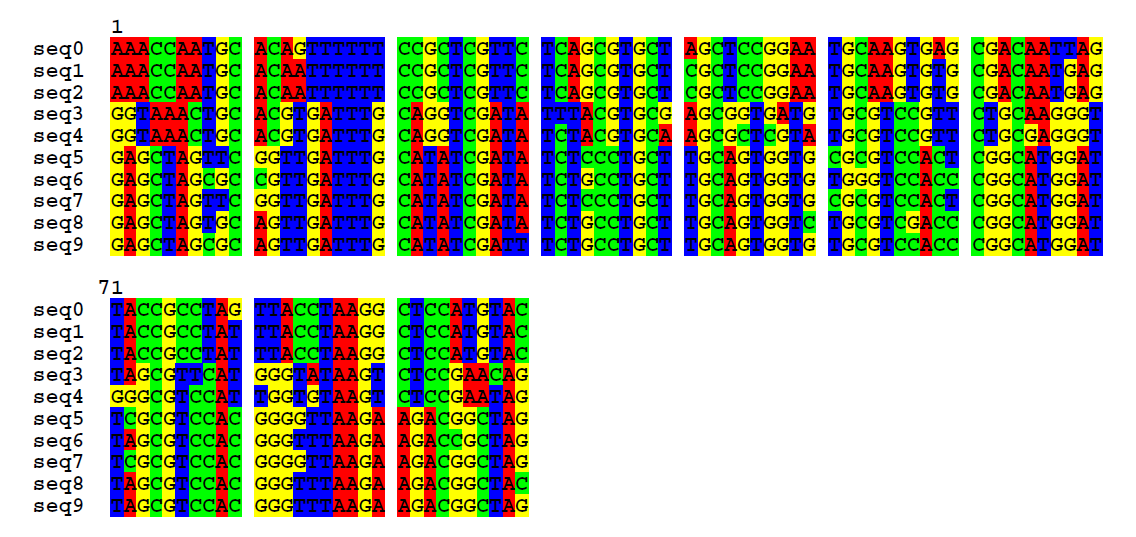
\includegraphics[width=\textwidth]{alignment1.png}
    \caption{An alignment generated by the previous command (\ref{cmd:1}). Two species are simulated, each with 5 sequences. The first species contains two populations; the first population has 3 sequences and the second population 2 sequences. The birth rate used to construct the phylogenetic tree is 2.0. Since, population 1 and population 2 of the first species merge at speciation time, they are as distant between themselves as the population of species 2. }
    \label{fig:4}
  \end{subfigure}
  
  
  \begin{subfigure}{\textwidth}
    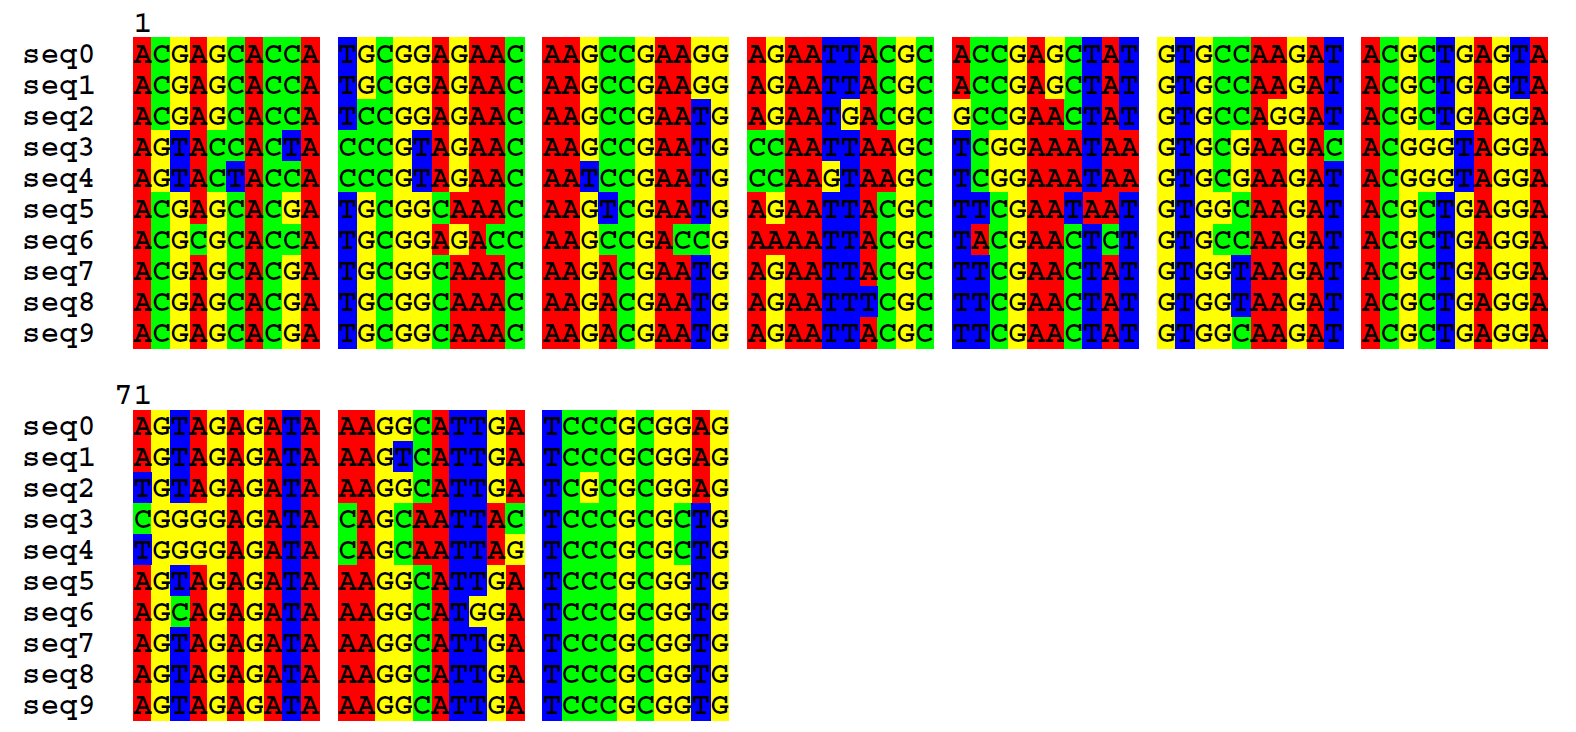
\includegraphics[width=\textwidth]{alignment2.png}
    \caption{An alignment generated by the previous command (\ref{cmd:2}). Two species are simulated, each with 5 sequences. The first species contains two populations; the first population has 3 sequences and the second population 2 sequences. The birth rate used to construct the phylogenetic tree is 10.0. In this simulation the population 1 merges with population 2 at a time which is older than the speciation event. In such a case, it is possible that either population 1 or population 2 is closer to population 3 (which belongs to species 2) than to each other. Here, population 1 is similar to population 3; population 2 is very different. }
    \label{fig:5}
  \end{subfigure}
\end{figure}




\subsection{Demographic events within species}
Within the boundaries of each species, demographic events may occur. All but the split event (\verb!-s!) of Hudson's ms can be implemented. Thus, species may have multiple populations, populations may change size and exchange genetic material (gene flow). Since there are more than one species to be simulated, the command line is partially different than Hudson's ms. The main difference is that the user can specify the species on which the ancestral event has taken place. 

\subsubsection{Population size changes}
The following command simulates a bottleneck within one of the species.

\begin{lstlisting}[label=cmd:3, caption={Command line to produce a bottleneck within one species}]{language=bash, label=cmd:3}
  ./comus 2 5 5 1 -eN 0.25 1 0.01 -eN 0.3 1 1.2 -t 10 -mm hky 
  -birth 2 -name example2 -ej 2.0 1 2 1 -oPhylo -oCoalescent
\end{lstlisting}

The code \ref{cmd:3} simulates a bottleneck that has occured at time 0.25 ($times 4 N_e$ generations). The population decreased by a factor of 100 and then at time 0.3 it increased by a factor of 1.2. The main difference with Hudson's ms is the specification of the species where the population size change took place (-eN 0.3 {\bf 1} 1.2). In this case \emph{all} populations of species 1 will experience the bottleneck. All population size changes are \emph{relative} to the first population of the first species (here denoted as $N0$). This is similar to Hudson's ms. 

In general the \verb!-eN! flag supports the following cases:

\begin{itemize}
\item \verb!-eN <time> <Nb>!: In this case all populations from all species will experience a population size change by a factor \verb!<factor>!
\item \verb!-eN <time> <species> <Nb/N0>!: All populations of species \verb!<species>! experienced a population size change. The modified population size was \verb!Nb/N0!, that took place at time \verb!<time>!.
\item \verb!-eN <time> <species> <population> <Nb/N0>!: Population \verb!<population>! of species \verb!<species>! experienced a population size change. The modified population size was \verb!Nb/N0!. 
\end{itemize} 

\subsubsection{Growth rate changes}
Similar to the population size changes, \comus\ can simulate growth rate changes. Thus, the following cases have been implemented:

\begin{itemize}
\item \verb!-eG <time> <growth rate>!: the growth rate for \emph{all} populations becomes \verb!<growth rate>! at time \verb!<time>!. 
\item \verb!-eG <time> <species> <growth rate>!: the growth rate for \emph{all} populations of species \verb!<species>! become \verb!<growth rate>! at time \verb!<time>!. 
\item \verb!-eG <time> <species> <population> <growth rate>!: the growth rate for population \verb!<population>! of species \verb!<species>! becomes \verb!<growth rate>! at time \verb!<time>!. 
\end{itemize}


\subsection{Migration (gene flow) events}
Migration has been also implemented in \comus. The following cases have been implemented:

\begin{itemize}
\item \verb!-migration <M>!: migration rate per population pair is $M$, i.e. the same for all population pairs.
\item \verb!-migration <species> <M>!: migration rate for each population pair of species species \verb!<species>!. In this case migration refers only to migration events that take place between the population of species \verb!<species>!.
\item \verb!-migration  <species 1> <species 2> <M>!: migration rate per each pair of populations of species \verb!<species 1>! and \verb!<species 2>!.
\item \verb!-migration <species 1> <population 1> <population 2> <M>!: migration rate between \verb!<population 1>! and \verb!<population 2>! of species \verb!<species>! is \verb!<M>!.
\item \verb!-migration <species 1> <population 1> <species 2> <population 2> <M>!: migration rate for \verb!<population 1>! and \verb!<population 2>! of species \verb!<species 1>! and \verb!<species 2>!, respectively is \verb!<M>!. 
\end{itemize}


\subsection{Joining population events}
\comus\ handles population joining events similar to Hudson's ms. Effectively, a joining event between a population $A$ and a population $B$ brings all lines of population $A$ to population $B$. The following cases have been implemented in \comus:

\begin{itemize}
\item \verb!-ej <time> <species 1> <population 1> <population 2>!: At time \verb!<time>! \\
\verb!<population 1>! joined \verb!<population 2>!
\item \verb!-ej <time> <species 1> <population 1> <species 2> <population 2>!: At time \verb!<time>! \verb!<population 1>! from species \verb!<species 1>! joins \verb!<population 2>! from species \verb!<species 2>!. 
\end{itemize}


\section{Partial isolation after a speciation event}
Typically, speciation events are considered to be instantaneous. However, after a speciation event it is possible that the daughter species are still able to exchange genetic material at least for some period of time. In \comus\ we have allowed to have partial isolation after a speciation event. 

\subsection{Implementing partial isolation events using heterogeneous Poisson processes}
Following a speciation event (forward in time) gene flow should gradually diminish between the two daughter species. Thus, the number of gene flow events and the time between the gene flow events can be modeled using a Poisson process. Such a process, however, will be inhomogeneous, because migration rate decreases over time until complete isolation. We can model such events using the inhomogeneous Poisson process and a rejection algorithm to draw times between events. 

The idea is has been described in several statistical textbooks (e.g. pg 32 in Ross' book `Simulation'). The algorithm is based on acceptance/rejection random numbers in such a way that the accepted values follow a non-homogeneous Poisson process with a specific rate. The pseudocode is shown in Code \ref{code:1}.

\begin{algorithm}
  %\KwResult{Time Intervals from a non-homogeneous Poisson Process}

  tis := \text{isolation time point}\;
  tsp := \text{speciation time point}\;
  cur := \text{current time}\;
  maxMig := \text{maximum migration rate}\;
  
  \While{true}{
    u $\sim U(0,1)$\;

    t := cur - (1/maxMig) $\times log(1-u)$\;

    v $\sim U(0,1)$\;

    \If{v \gt t/(tsp - tis) - tis/(tsp - tis) } 
    {break}
  }
  \Return t - cur
  
  \vspace{5pt}
  
  \caption{Producing time intervals from an non-homogeneous Poisson Process}
  
  \label{code:1}

\end{algorithm}


To run simulations with partial isolation, the user has to specify the following flags on the command line:

\begin{itemize}
\item \verb!-partIsolation!:  this flag switches on the partial isolation model.
\item \verb!-partIsoPeriod <float>!: The time interval after a speciation event for which the daughter species are only partially isolated.
\item \verb!-partMaxMigration <float>!: The maximum migration rate (i.e. gene flow at the moment of speciation)
\end{itemize}

Figure \ref{fig:6} illustrates the parameters used for the partial isolation model.



\begin{figure}[htbp!]
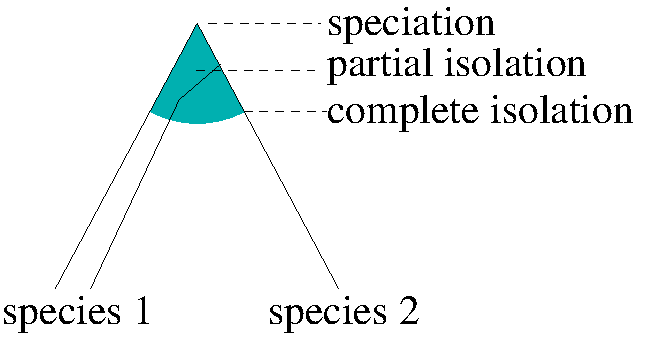
\includegraphics[width=0.9\textwidth]{partial_isolation.pdf}
\caption{A coalescent tree for two species demonstrating the partial isolation after speciation model. Species 1 consists of two sequences (on the left of the tree), whereas species 2 consists of one sequence. Speciation occurred at the root of the tree. There is a period of time, after speciation, where species are not yet completely isolated (blue interval). Thus, it is possible that coalescent between lineages of species 1 and species 2 will occur during this time interval. Indeed, the second lineage of species 1 coalesces with the lineage of species 2 during the partial isolation period. }
\label{fig:6}

\end{figure}

An example command line that demonstrates the partial isoloation model is the following:


\begin{lstlisting}[label=cmd:4, caption={Command line to simulate under the partial isolation model}]{language=bash, label=cmd:4}
  
  ./comus 4 1 1 1 1 10 -t 10 -r 2  -rsites 100 -mm hky 
  -msites 100 -name run -oPhylo -oCoalescent -birth 100  
  -partIsolation -partIsoPeriod 1.0 -partMaxMigration 10 -oPhylo

\end{lstlisting}

Command line \ref{cmd:4} will produce 10 independent simulations for 4 species. Each species has one sequence and speciation occurs gradually (i.e. partial isolation after speciation). The isolation period after each speciation event is 1 (time is measured in the usual phylogenetic units), and the maximum migration rate (i.e. at the time of speciation) is 10. 


\section{Ancestral sampling}
Ancestral sampling has been implemented in CoMuS either for populations or species. That means that currently it is not possible to sample individuals from the same population at different time points. 
The key steps behind the implementation of ancestral sampling are the following:

\begin{itemize}
\item  Sample all individuals at time 0, i.e., present. Thus, initially, all individuals are considered to be present-day samples.
\item Do not allow any event take place between the present and sampling time for individuals of species that are sampled in the past, i.e., no coalescent, recombination, migration from and to, speciation, etc are allowed.  Thus, if an event is going to happen that involves a line that `has not been sampled yet', then the event is rejected and a new event takes place. This simple approach guarantees that waiting times for all events are drawn from a proper distribution. After sampling (backward in time) all these processes take place as usual. 
\end{itemize}

For example, if during the construction of coalescent tree, the next event is going to happen is a recombination event in population $P$ at time $t$, then we first check whether sampling time of population $P$ is before $t$. If this not the case, then $P$ has not been sampled yet, so no event can take place. For example, the code in the \verb!comus_streec.c! is:

\begin{lstlisting}
if( samplingTime[ chrom[ ic ].pop ] <= t )
{
   eventOccured = 1;
   rchrom = re2(nsam, ic, is);                                                                            
   config[ chrom[rchrom].pop ] += 1 ;
}
\end{lstlisting}

The `if' statement controls whether current time is greater or equal to the sampling time (we are moving towards the past). An event (in this case recombination) is allowed to take place only when it is older than the sampling time. 

\begin{itemize}
\item After coalescent has been completed set the time of the leaves that have sampled in the past, at sampling time. This will guarantee that mutations will happen correctly. 
\end{itemize}

Figure~\ref{ancestral} illustrates how ancestral sampling is implemented for species 1 (ind1, ind2, ind3, ind4, ind5). 

\subsection{Modes of ancestral sampling}
Ancestral sampling can be invoked with different ways, depending on whether we have sampled one species (and all its populations) or a specific population in the past. The following ways are possible:

\begin{itemize}
\item \verb!-samplingtime <float TIME>! This sets the sampling time for all individuals (from all species and populations) to \verb!TIME!. 
\item \verb!-samplingtime <int SPECIES> <float TIME>! This sets the sampling time for all individuals of species \verb!SPECIES! to time \verb!TIME!. 
\item \verb!-samplingtime <int SPECIES> <int POP> <float TIME>! This sets the sampling time for all individuals of population \verb!POP! of species \verb!SPECIES! at \verb!TIME!. 
\end{itemize}


\begin{figure}
\centering

\caption{}
\label{ancestral}

\end{figure}




\chapter{Examples}

\section{ms-like commands}

\begin{lstlisting}[label=cmd:5, caption={Simple ms command}]{language=bash}
  ./comus 10 1 -t 10 -r 10 100
\end{lstlisting}

Command \ref{cmd:5} produces polymorphisms from 10 sequences. $\theta = 10$, $\rho = 10$ and there exist 100 potential breakpoints. 


\begin{lstlisting}[label=cmd:6, caption={ms command with two populations}]{language=bash}
  ./comus 10 1 -I 2 5 5 -t 1 -r 10 100 -ej 5.2 2 1
\end{lstlisting}

Command \ref{cmd:6} produces polymorphisms for 10 sequences, which have been sampled from two populations. Populations are isolated until time point 5.2 (time is measured in coalescent units). 

\section{multiple species examples}

When multiple species are simulated, then please note the following:
\begin{itemize}
\item You need to {\bf provide a name for the run}. i.e. use the flag -name. This is needed because \comus\ is producing several output files, and for each of them it is using the `name' as a suffix. 
\item If you plan to use the finite site model, then use the flag {\bf -mm}. Then, you must provide the mutation model. \comus\ is using the same mutation models as Rambaut's Seq-Gen.
\end{itemize}

\begin{lstlisting}[label=cmd:7, caption={Two species, random phylogenetic tree}]{language=bash}
  ./comus 2 10 10 1 -t 10 -birth 5 -r 10 -rsites 10 
  -msites 100 -mm hky -name example3
\end{lstlisting}

Command line \ref{cmd:7} will produce 1 simulation. 
\begin{itemize}
\item The first integer specifies the number of species (i.e. 2)
\item Then (10 10) is the sample size for each species
\item The fourth integer (i.e. 1) is the number of replications. 
\item Then, it come $\theta$ (-t 10). Mutation rate is scaled according the population size of the first population, and the first species as in Hudson's ms. 
\item The flag -birth specifies the birth rate for the simulation of the guide species tree.
\item Then, the recombination rate is specified (-r 10). 
\item Then, the number of sites that can recombine ( -rsites 10). In the original ms this was -r 10 10. However, I find it confusing when it is used together with the -msites (see below). Thus, I decided to denote explicitly that -rsites is the number of the recombining sites. 
\item Then, the number of sites (that can be mutated) is given (-msites). This is needed for the finite site model. Thus, we do not obtain results based on the infinite site model, but a sequence of a specified length is simulated. 
\item The next flag (-mm hky) specifies the mutation model (i.e. HKY); here we use default parameters. See the manual of seq-gen for additional information. 
\item The last flag specifies the name of the run. The output files will have as a suffix the `example3', since this is the name of the run. 
\end{itemize}


The command \ref{cmd:8} simulates an alignmemnt of four sequences; each sequence belongs to a separate species. In detail:

\begin{lstlisting}[label=cmd:8, caption={Two species, user-defined phylogenetic tree}]{language=bash}
  ./comus 4 1 1 1 1 2 -t 10 -iphylo tree.newick2 -mm hky -msites 100 
  -name example5 -oPhylo -oCoalescent   -partIsolation 
  -partIsoPeriod 0.50 -partMaxMigration 500.0  -G 100
\end{lstlisting}


\begin{itemize}
\item \code{comus 4 1 1 1 1 2} specifies a simulation of 4 species, each one with 1 sequence. There will be 2 replications.
\item \code{-t 10} specifies the population mutation rate
\item \code{-iphylo tree.newick2} imports the guide phylogenetic tree. The tree format is newick. Specifically, the tree is given by:\\
\code{((1:0.1, 2:0.1):0.2, (3:0.2, 4:0.2):0.1);}. 
\item \code{-mm hky}: specifies the mutation model (default parameters).
\item \code{-msites 100} is the length of the sequence (finite site model)
\item \code{-name example5} is the name of the run and this will be the suffix for the produced files
\item \code{-oPhylo} outputs the phylogenetic tree
\item \code{-oCoalescent} outputs the coalescent tree(s)
\item \code{-partIsolation -partIsoPeriod 0.50 -partMaxMigration 500} refer to the partial isolation model
\item \code{-G 500} sets initial growth rates for \emph{all} populations
\end{itemize}






